\documentclass[12pt]{article}

\usepackage[utf8]{inputenc}
\usepackage[russian]{babel}
\usepackage{graphicx}
\usepackage{indentfirst}
\usepackage{booktabs}


\graphicspath{{pic/}}

\begin{document}

\begin{center}
	\LARGE 
	\textbf{Практическое занятие 3}\\
	ПРОГРАММИРОВАНИЕ В СРЕДЕ MATLAB\\
\end{center}

\begin{flushright}
	\large
	Игнашов Иван\\
	Вариант 8\\
\end{flushright}

\newpage

 \section*{1. Цель работы}
Изучение реализации средствами системы MATLAB основных операций с векторами и матрицами.
\subsection*{Порядок работы:}
\begin{enumerate}
	\item Из файла-сценария с помощью функции диалогового ввода ввести с клавиатуры все необходимые данные. Выполнить расчет с использованием условных операторов и вывести результаты в командное окно\\
		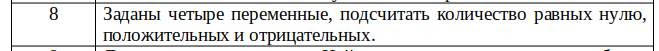
\includegraphics[width=0.75\linewidth]{formula.png}
	\item Написать файл-функцию с использованием операторов ветвления и циклов\\
		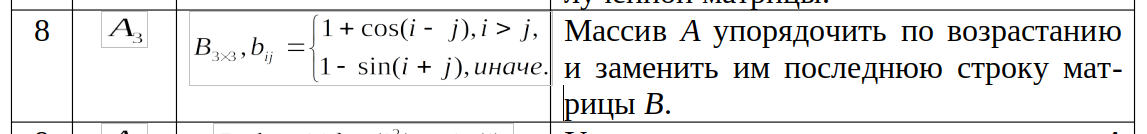
\includegraphics[width=0.75\linewidth]{formula2.png}
\end{enumerate}

\newpage
 \section*{2. Листинг программ и результаты выполнения программ}%
 
 \subsection*{2.1. файл-сценарий}
 
 \begin{figure}[!h]
	\centering
	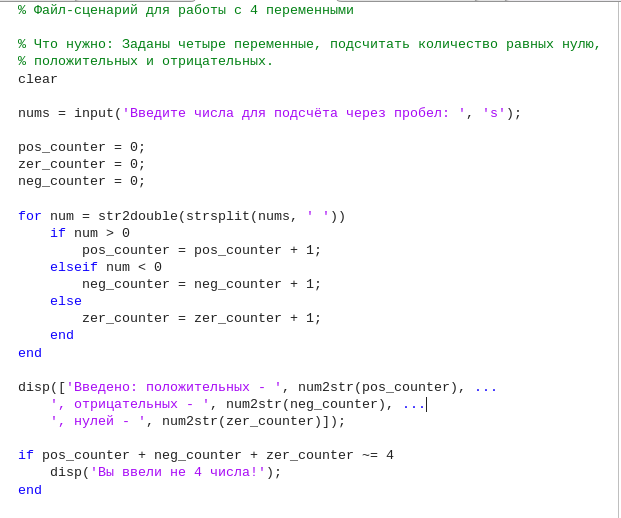
\includegraphics[width=\linewidth]{file_procedure.png}
	\caption{Сценарий - обработка переменных}
\end{figure}
Для упрощения ввода и считывания переменных было решено считать все числа строкой, а потом разделить их по символу пробела. Так как после разделения пробелом строки получается вектор, то в цикле \textbf{for} можно итерироваться прямо по нему

 \begin{figure}[!h]
	\centering
	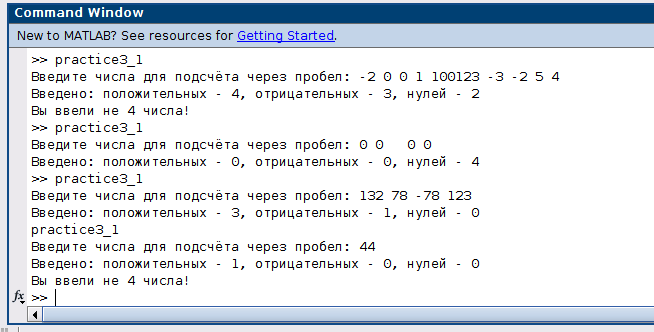
\includegraphics[width=\linewidth]{procedure_run.png}
	\caption{Примеры работы}
\end{figure}
\begin{figure} 
 \subsection*{2.2. файл-функция}
\end{figure}
\begin{figure}[!h]
	\centering
	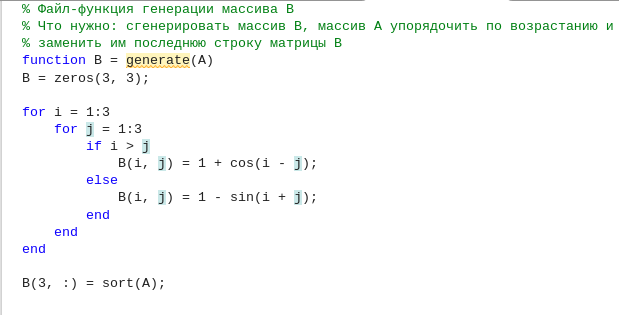
\includegraphics[width=\linewidth]{file_function.png}
	\caption{Функция - генерация матрицы 3х3}
\end{figure}

\begin{figure}[!h]
	\centering
	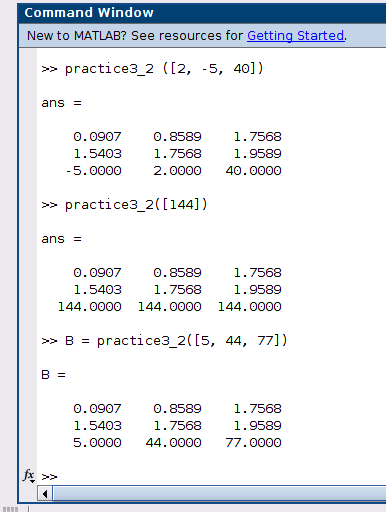
\includegraphics[width=0.6\linewidth]{function_run.png}
	\caption{Примеры работы}
\end{figure}

\begin{figure}
При присваивании скаляра \textit{(вызов practice3-2([144])} строке матрицы видно, что matlab присвоил этот скаляр всем элементам строки
\end{figure}

\end{document}